\chapter{Experiments}
\section{TIMIT}
The \textit{timit} speech corpus \cite{Garofolo1993}, contains recordings of ten phonetically rich sentences, for example:
\begin{quotation}
\textquotedblleft She had your dark suit in greasy wash water all year. \textquotedblright
\end{quotation}
For each sentence a transcription of the spoken phonemes is also available. Phonemes are sets of sounds, which
are considered equivalent in a given language. In alphabetic writing systems one the phoneme to letter mappings should ideally be bijective. Bijective functions map one input to only one target and vice versa. Due to the fact that the Latin script was devised for classical Latin as well as the fact that when pronunciation changes the spelling often remains the same, the phoneme to letter mappings are often far from ideal in modern languages. Therefore the \texttt{timit} data set comes with phonetic transcriptions for all sentences. For the sentence considered above the spoken phonemes are:
\begin{quotation}
\textquotedblleft h\# sh ix hv eh dcl jh ih dcl d ah kcl k s ux q en gcl g r ix s ix w ao sh epi w ao dx axr ao l y ih axr h\# \textquotedblright
\end{quotation}
The transcriptions contain a total of 64 possible phonetic labels, in the literature the full set and foldings with 48 and 39 labels are considered \cite{Lee1989}. In all following experiments the 39 labels shown in \ref{fig:phoneTable} will be considered.

\begin{figure}
\centering
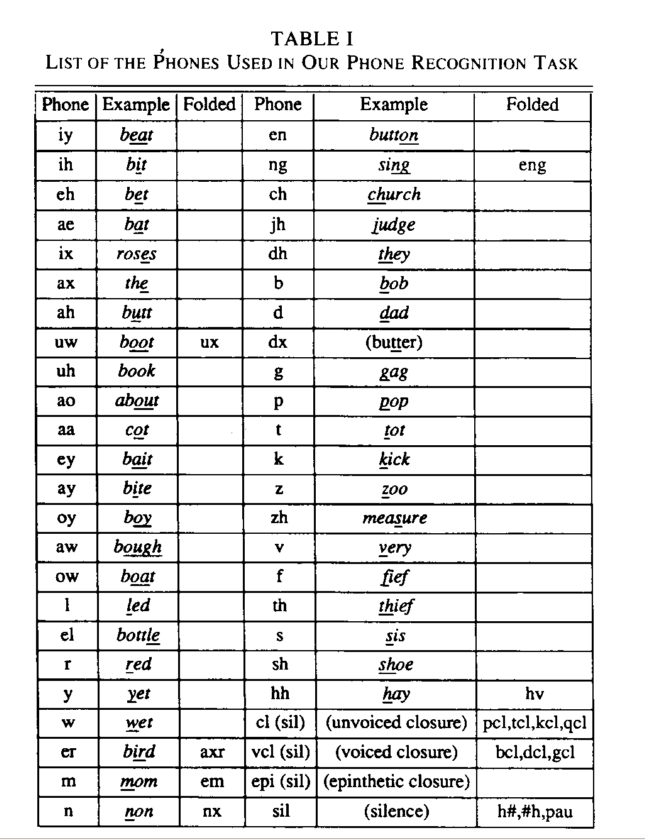
\includegraphics[width=0.7\linewidth]{png/phoneTable}
\caption{48 to 39 phoneme folding as shown in \cite{Lee1989}.}
\label{fig:phoneTable}
\end{figure}

The timit data set is split into a training, validation and test set. Containing 3696, 400 and 192 sentences \cite[page  80]{Graves2012}.


\section{BLSTM-CTC}
\begin{figure}
\centering
\includestandalone[width=0.49\linewidth]{tikz/faem0si2022wav}
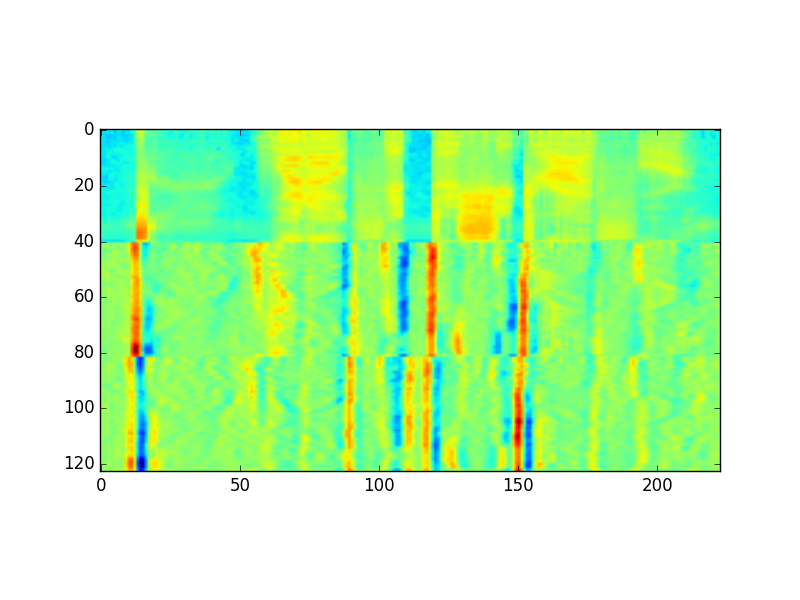
\includegraphics[width=0.49\linewidth]{png/feats_faem0_si2022.png}
\caption{Raw time domain signal and feature vectors. Features include 40 mel banks as well as the first and second derivatives. Raw data was taken from TIMIT utterance faem0-si2022 \enquote{What outfit does she drive for?}.}
\label{fig:timitFeats}
\end{figure}

This section explores bidirectional long short term memory layers with CTC output on the timit corpus \cite{Graves2012, Graves2006}. Training began after transforming of the speech data into Mel frequency cepstral coefficients (\textit{MFCCC}s) augmented with first and second derivative information. The raw time domain signal as well as the feature vectors are shown in figure~\ref{fig:timitFeats}. The phonemes where folded as described above. Two \textit{BLSTM} layers where stacked on top of each other, both using LSTM cells with a dimension of 64 in each direction. The logits computed by the two layers where then fed into a CTC output layer, finally beam search decoding with a beam width of 100 was used to find the phoneme predictions. The whole network was optimized using gradient descent and a learning rate of $10^{-3}$. To ensure generalization normal input noise $\mathcal{N}(\mu = 0,\sigma = 0.65)$ was added to the inputs. All feed-forward weights where initialized using another Gaussian $\mathcal{N}(0, 0.1)$, lstm weights were initialized using a random uniform distribution $\mathcal{U}(-0.1, 0.1)$. Gradients where clipped such that all gradient elements are within $(-1,1)$.
\begin{figure}
\centering
\includestandalone[width=0.49\linewidth]{tikz/CTC_Listener_plot_e10_no_pyramid_loss}
\includestandalone[width=0.49\linewidth]{tikz/CTC_Listener_plot_e10_no_pyramid_error}
\caption{Validation and Test set error while training a two layer BLSTM network with CTC output layer on the TIMIT speech corpus with 39 folded phonemes.}
\label{fig:ctc2BLSTM41}
\end{figure}
Results of the training process are shown in figure~\ref*{fig:ctc2BLSTM41}. In the experiment the training process was stopped after 10 epochs to be able to compare the result to the pyramidal listener experiment in the next chapter, at this point the phoneme error rate of this layout was at $29\%$. However if the training process is continued with decreasing learning rates the error rate values end up close to $26\%$ eventually. Performance can be increased further by assigning the LSTM cells a larger state dimension.











